% ================================================================
% Unified Paper — NeurIPS 2026
% "From Situational to Unconditional: The Spectrum of Moral
%  Commitment Required for Multi-Agent Survival in Non-linear
%  Social Dilemmas"
% ================================================================
\documentclass{article}
\usepackage[preprint]{neurips_2026}
\usepackage[utf8]{inputenc}
\usepackage[T1]{fontenc}
\usepackage{amsmath,amssymb,amsfonts,amsthm}
\usepackage{hyperref}
\usepackage{url}
\usepackage{booktabs}
\usepackage{nicefrac}
\usepackage{microtype}
\usepackage{xcolor}
\usepackage{graphicx}

\newtheorem{theorem}{Theorem}
\newtheorem{proposition}{Proposition}
\newtheorem{definition}{Definition}

\title{From Situational to Unconditional:\\The Spectrum of Moral Commitment Required for\\Multi-Agent Survival in Non-linear Social Dilemmas}

\author{Anonymous Author(s)}

\begin{document}
\maketitle

% ================================================================
% ABSTRACT
% ================================================================
\begin{abstract}
When must multi-agent systems move beyond self-interest, and how much moral commitment is enough?
We investigate this question by computationally instantiating Amartya Sen's meta-ranking theory---where agents' commitment level $\lambda_t$ dynamically adapts to resource availability---in Public Goods Games of increasing environmental severity.
In \emph{linear} PGG environments (moderate recovery dynamics), \textbf{situational commitment}---where agents reduce prosocial behavior during resource crises to preserve survival---achieves group-level evolutionary stability (ESS) via multi-level selection ($\bar{x}=0.987$), outperforming selfish, deontological, and opponent-shaping baselines across 8 environments.
However, when we extend the environment to include \emph{non-linear tipping points}---irreversible collapse below $R_{\text{crit}}$---situational commitment catastrophically fails.
Purely selfish MAPPO agents converge to a \emph{Nash Trap} at $\lambda \approx 0.5$, with survival dropping to 5.3\% under 30\% Byzantine adversaries.
Parameter optimization reveals that only \textbf{unconditional commitment} ($\phi_1^* = 1.0$) prevents collapse, improving bottom-10\% welfare by +587 points while maintaining structural immunity to adaptive adversaries ($<$1.3\% welfare reduction).
Notably, decentralized intrinsic-motivation baselines---Inequity Aversion and Social Influence---achieve \textbf{0\% survival} under Byzantine conditions, as agents observing adversaries' zero contributions adaptively reduce their own, accelerating collective collapse.
Our central finding is a \textbf{Moral Commitment Spectrum}: the degree of commitment required for system survival is determined by the environment's non-linearity.
Moderate environments permit flexible, survival-aware morality; catastrophic environments demand unconditional sacrifice---an engineering necessity, not a philosophical preference.
\end{abstract}

% ================================================================
% SECTION 1: INTRODUCTION (Act 1)
% ================================================================
\section{Introduction}

Rational Choice Theory defines human behavior as utility maximization under constraints.
\citet{sen1977rational} critiqued this as the ``Rational Fool,'' arguing that genuine moral behavior requires \textit{commitment}---acting against immediate self-interest---mediated through \textit{meta-rankings}: preferences over preference orderings.
This philosophical insight gains urgent practical relevance as multi-agent reinforcement learning (MARL) systems are increasingly deployed in domains exhibiting \textbf{non-linear dynamics and tipping points}---climate systems, financial markets, and ecological networks~\citep{lenton2008tipping}---where the failure to cooperate can trigger irreversible collapse.

Can self-interested agents discover cooperative strategies through reward maximization alone, or must cooperation be architecturally encoded?
And if moral commitment is necessary, \emph{how much} commitment does the environment demand?

We address these questions through a systematic investigation spanning environments of increasing severity, yielding four contributions:
\begin{enumerate}
    \item[(C1)] \textbf{Computational Instantiation of Sen's Meta-Ranking}: We formalize commitment as a dynamic parameter $\lambda_t \in [0,1]$ that adapts to resource state $R_t$ and Social Value Orientation $\theta_i$, enabling agents to balance self-interest and prosocial behavior (Section~\ref{sec:method}).
    \item[(C2)] \textbf{Situational Commitment Works in Linear Environments}: In standard PGG with moderate recovery dynamics, resource-conditioned commitment achieves group-level ESS ($\bar{x}=0.987$), outperforming 8 baselines including M-FOS and POLA (Section~\ref{sec:linear}).
    \item[(C3)] \textbf{The Nash Trap in Non-linear Environments}: When tipping points introduce irreversible collapse, both situational commitment and pure RL (MAPPO) fail---agents converge to $\lambda \approx 0.5$, insufficient to prevent catastrophe (Section~\ref{sec:nash_trap}).
    \item[(C4)] \textbf{Unconditional Commitment as Engineering Necessity}: Only maximal crisis commitment ($\phi_1^* = 1.0$) guarantees system survival under adversarial conditions, while same-class decentralized baselines (Inequity Aversion, Social Influence) achieve 0\% survival---their \emph{other-regarding} mechanisms cause downward drift toward adversaries' zero contributions (Section~\ref{sec:unconditional}).
\end{enumerate}

Together, these results establish a \textbf{Moral Commitment Spectrum}: the severity of environmental non-linearity determines the minimum commitment required for collective survival.

% ================================================================
% SECTION 2: RELATED WORK
% ================================================================
\section{Related Work}

\paragraph{Social Dilemmas in MARL.}
The tension between individual and collective rationality has been studied in matrix games~\citep{leibo2017multi} and sequential social dilemmas~\citep{hughes2018inequity}.
Intrinsic motivation approaches---inequity aversion~\citep{hughes2018inequity}, social influence~\citep{jaques2019social}, reputation mechanisms~\citep{anastassacos2020cooperation}---promote cooperation but implicitly encode cooperative preferences, making it impossible to distinguish genuine emergence from training conditioning.

\paragraph{Opponent Shaping.}
LOLA~\citep{foerster2018learning} differentiates through opponent updates to shape learning in 2-player games.
M-FOS~\citep{lu2022model} extends this model-free via meta-learning, and POLA~\citep{zhao2022proximal} adds proximal regularization.
However, these methods require white-box access to opponent parameters and scale poorly beyond pairwise settings---LOLA diverges entirely at $N=50$.
Our framework requires only publicly observable resource levels.

\paragraph{Non-linear Dynamics and Tipping Points.}
While common-pool resource games have been studied~\citep{ostrom1990governing}, most MARL benchmarks use linear or stationary environments.
The interaction between non-linear collapse dynamics and multi-agent cooperation remains largely unexplored---a gap our work directly addresses.

% ================================================================
% SECTION 3: METHOD (Act 1 continued)
% ================================================================
\section{Method}
\label{sec:method}

\subsection{Meta-Ranking Reward Function}

\begin{definition}[Meta-Ranking Agent]
Agent $i$ with SVO angle $\theta_i$ maximizes:
\begin{equation}
R_{\text{total}}^{(i)} = (1 - \lambda_t^{(i)}) \cdot U_{\text{self}}^{(i)} + \lambda_t^{(i)} \cdot \left[ U_{\text{meta}}^{(i)} - \psi^{(i)} \right]
\label{eq:reward}
\end{equation}
\end{definition}
where $U_{\text{meta}}^{(i)} = \frac{1}{N-1}\sum_{j \neq i} U_{\text{self}}^{(j)}$ captures sympathy and $\psi^{(i)} = \beta |U_{\text{self}} - U_{\text{meta}}|$ models restraint cost.

\subsection{Dynamic Commitment Mechanism}

The key innovation is that $\lambda_t$ adapts to resource level $R_t$:
\begin{equation}
\lambda_t^{(i)} = \alpha \lambda_{t-1}^{(i)} + (1-\alpha) \cdot g(\theta_i, R_t)
\label{eq:lambda}
\end{equation}
where $g(\theta, R) = \begin{cases}
\max(0, \sin\theta \cdot 0.3) & R < R_{\text{crisis}} \\
\min(1, 1.5\sin\theta) & R > R_{\text{abundance}} \\
\sin\theta \cdot (0.7 + 1.6R) & \text{otherwise}
\end{cases}$

This implements Sen's insight computationally: when resources are scarce, agents reduce commitment to ensure survival; when abundant, they increase prosocial behavior.

\subsection{Environment Suite}
\label{sec:env}

\paragraph{Linear PGG.}
$N$ agents each receive endowment $E$ and contribute $c_t^i = E \cdot \lambda_t^i$.
Individual payoff: $r_t^i = (E - c_t^i) + M \sum_j c_t^j / N$ with multiplier $M = 1.6$.
Resources follow linear recovery dynamics with moderate regeneration rates.

\paragraph{Non-linear PGG with Tipping Points.}
We extend the linear environment with catastrophic collapse dynamics:
\begin{equation}
R_{t+1} = \text{clip}\!\left(R_t + f(R_t) \cdot \left(\bar{c}_t / E - 0.4\right) - \xi_t,\; 0,\; 1\right)
\label{eq:resource}
\end{equation}
where $\xi_t \sim \text{Bernoulli}(p_{\text{shock}}) \cdot \delta_{\text{shock}}$ represents exogenous shocks and $f(R_t)$ introduces a \textbf{tipping point}:
\begin{equation}
f(R_t) = \begin{cases}
0.01 & R_t < R_{\text{crit}} \quad \text{(near-irreversible collapse)} \\
0.03 & R_{\text{crit}} \leq R_t < R_{\text{recov}} \quad \text{(hysteresis)} \\
0.10 & R_t \geq R_{\text{recov}} \quad \text{(normal recovery)}
\end{cases}
\label{eq:tipping}
\end{equation}
with $R_{\text{crit}} = 0.15$ and $R_{\text{recov}} = 0.25$.
When $R_t \leq 0$, the episode terminates and all future rewards become zero.

% ================================================================
% SECTION 4: EXPERIMENTS
% ================================================================
\section{Experiments}

\subsection{Act 2: Situational Commitment in Linear Environments}
\label{sec:linear}

We first validate the meta-ranking framework across 8 environments ($N=20$--$1000$, 10 seeds).

\paragraph{Moral Theory Comparison.}
\begin{table}[t]
\centering
\caption{Moral theory comparison (linear PGG, $N{=}50$, 10 seeds).}
\label{tab:moral}
\begin{tabular}{lcccr}
\toprule
Theory & Coop & Welfare & Sustain. & ESS\% \\
\midrule
Utilitarian & 1.000 & 147.7 & 100\% & 99.6\% \\
\textbf{Situational (Ours)} & 1.000 & 147.7 & 100\% & 0.1\% \\
Deontological & 1.000 & 129.7 & 100\% & 0.1\% \\
Virtue Ethics & 0.684 & 118.9 & 100\% & 0.1\% \\
Selfish & 0.000 & 102.8 & 26\% & 0.1\% \\
\bottomrule
\end{tabular}
\end{table}

Table~\ref{tab:moral} demonstrates that Situational Commitment matches Utilitarian welfare while using only local resource information---no global welfare oracle required.

\paragraph{SOTA Comparison.}
We compare against 4 representative opponent-shaping and reward-shaping baselines (Table~\ref{tab:sota}).

\begin{table}[t]
\centering
\caption{SOTA comparison (linear PGG, $N{=}50$, 10 seeds). ``Byz'' = cooperation under 50\% Byzantine adversaries. ``Decentr.'' = no opponent parameter access required.}
\label{tab:sota}
\begin{tabular}{lcccccc}
\toprule
Method & Coop & Welfare & Gini & Byz & Decentr. \\
\midrule
M-FOS & 1.000 & 156.3 & 0.000 & 0.143 & \texttimes \\
POLA & 1.000 & 148.3 & 0.000 & 0.504 & \texttimes \\
LOLA & 0.000 & 101.5 & 0.014 & 0.000 & \texttimes \\
LOPT & 0.000 & 101.4 & 0.014 & 0.000 & \texttimes \\
\textbf{Meta-Ranking (Ours)} & 1.000 & 148.0 & 0.011 & \textbf{0.500} & \checkmark \\
\bottomrule
\end{tabular}
\end{table}

\noindent\textit{Key finding}: M-FOS achieves the highest benign welfare ($156.3$) via meta-learning opponent shaping, but collapses under Byzantine adversaries ($0.143$).
POLA maintains $0.504$ Byzantine cooperation, matching meta-ranking's $0.500$, but requires white-box access to opponent parameters---precluding decentralized deployment.
Meta-ranking is the only method simultaneously achieving high Byzantine resilience and full decentralization.

\noindent\textit{Architectural Note}: We emphasize that the computational advantage of meta-ranking over opponent-shaping methods reflects a fundamental \emph{architectural difference}, not an algorithmic optimization.
Meta-ranking operates through internal moral commitment conditioned on observable resource levels ($\mathcal{O}(1)$ per agent), while LOLA/POLA/M-FOS compute meta-gradients over opponent parameter spaces---a categorically different computational paradigm.
Direct speed comparisons across these paradigms would be misleading; the relevant distinction is that meta-ranking \emph{requires no opponent modeling}, making it uniquely suited for decentralized, privacy-preserving deployment.

\paragraph{Group-Level Evolutionary Stability (Theorem~\ref{thm:group_ess}).}

\begin{theorem}[Group-Level ESS via Price Equation]
\label{thm:group_ess}
Under group replacement dynamics with migration rate $m < m^* = \Delta p_{\text{between}} / (|\Delta p_{\text{within}}| + \Delta p_{\text{between}})$, Situational Commitment achieves group-level evolutionary stability. Specifically:
$\Delta p_{\text{within}} = -0.115$ (within-group free-riding advantage),
$\Delta p_{\text{between}} = +0.046$ (between-group fitness advantage, 58.2\% group welfare gain).
Population convergence: $\bar{x} = 0.987$ after 100 generations.
\end{theorem}

\noindent The critical constraint $m < m^*$ ensures that inter-group mixing does not erode the between-group selection advantage.
Full proof with ecological boundary conditions is provided in Appendix~\ref{app:price}.

\subsection{Act 3: The Turning Point---Non-linear Extension}
\label{sec:turning_point}

Having established that situational commitment succeeds in linear environments, we now ask: \emph{does it survive when the environment introduces catastrophic tipping points?}

We deploy the same meta-ranking agents in the non-linear PGG (Equations~\ref{eq:resource}--\ref{eq:tipping}) with $R_{\text{crit}} = 0.15$, stochastic shocks ($p_{\text{shock}} = 0.05$, $\delta_{\text{shock}} = 0.15$), and 30\% Byzantine adversaries.

\textbf{Result: Situational commitment fails catastrophically.}
When resources drop below $R_{\text{crit}}$, the commitment function $g(\theta, R)$ reduces $\lambda$ to $\max(0, \sin\theta \cdot 0.3)$---precisely when maximum commitment is needed to overcome the near-irreversible recovery dynamics ($f(R_t) = 0.01$).
The very survival mechanism that was adaptive in linear environments becomes suicidal in non-linear ones: reducing commitment during crises \emph{accelerates} passage through the tipping point.

This discovery motivates two questions: (1) Can pure RL find a better strategy without any pre-specified commitment? (2) What level of crisis commitment is actually required?

\subsection{Act 4: The Nash Trap---Failure of Selfish RL}
\label{sec:nash_trap}

\paragraph{MAPPO with Pure Selfish Payoff.}
We train MAPPO agents with \emph{only} individual payoff as reward---no reward shaping, no intrinsic motivation, no social priors.
Each agent observes $s_t^i = (R_t, \bar{c}_{t-1}/E, \lambda_{t-1}^i, \mathbb{1}[R_t < R_{\text{crit}}])$ and outputs:
\begin{equation}
\lambda_t^i = \text{clip}\!\left(\sigma(w^\top s_t^i + b) + \epsilon_t,\; 0,\; 1\right), \quad \epsilon_t \sim \mathcal{N}(0, \sigma_{\text{noise}}^2)
\end{equation}
with annealed exploration ($\sigma_{\text{noise}}$: $0.15 \to 0.02$).

\begin{table}[t]
\centering
\caption{RL emergence test (non-linear PGG, $N{=}20$, 5 seeds).}
\label{tab:emergence}
\begin{tabular}{lcccc}
\toprule
\textbf{Method} & \textbf{Welfare} & $\boldsymbol{\bar{\lambda}}$ & \textbf{Survival \%} & \textbf{Crisis $\boldsymbol{\lambda}$} \\
\midrule
MAPPO (selfish) & 26.0 & 0.500 & 83.3 & 0.501 \\
MAPPO + Byz 30\% & 24.2 & 0.500 & \textbf{5.3} & 0.500 \\
\midrule
Fixed $\lambda=0.0$ & 20.0 & 0.000 & 0.0 & --- \\
Fixed $\lambda=0.5$ & 26.0 & 0.500 & 87.3 & --- \\
Fixed $\lambda=1.0$ (oracle) & \textbf{32.0} & 1.000 & \textbf{100.0} & --- \\
\bottomrule
\end{tabular}
\end{table}

\textbf{Result}: RL agents converge to $\lambda \approx 0.5$ regardless of crisis state (crisis $\lambda = 0.501 \approx \bar{\lambda}$).
Policy weights remain near zero ($|W| < 0.01$): the REINFORCE gradient vanishes at this equilibrium.
Under 30\% Byzantine adversaries, survival plummets to \textbf{5.3\%} (Table~\ref{tab:emergence}).
Critically, this result holds at $N=100$ (Table~\ref{tab:scale}), confirming the Nash Trap is a game-theoretic property, not a small-$N$ artifact.

\begin{table}[t]
\centering
\caption{Scale test: Nash Trap persists at $N{=}100$ (non-linear PGG, 5 seeds, 50 episodes).}
\label{tab:scale}
\begin{tabular}{lccc}
\toprule
\textbf{Method ($N{=}100$)} & \textbf{Welfare} & $\boldsymbol{\bar{\lambda}}$ & \textbf{Survival \%} \\
\midrule
Selfish RL (Byz=0\%) & 26.0 & 0.500 & 86.4 \\
Selfish RL (Byz=30\%) & 24.2 & 0.500 & \textbf{10.4} \\
\midrule
Situational (Byz=30\%) & 27.5 & 0.897 & 99.6 \\
Unconditional (Byz=30\%) & 26.6 & 0.790 & 93.6 \\
\bottomrule
\end{tabular}
\end{table}

\begin{figure}[t]
    \centering
    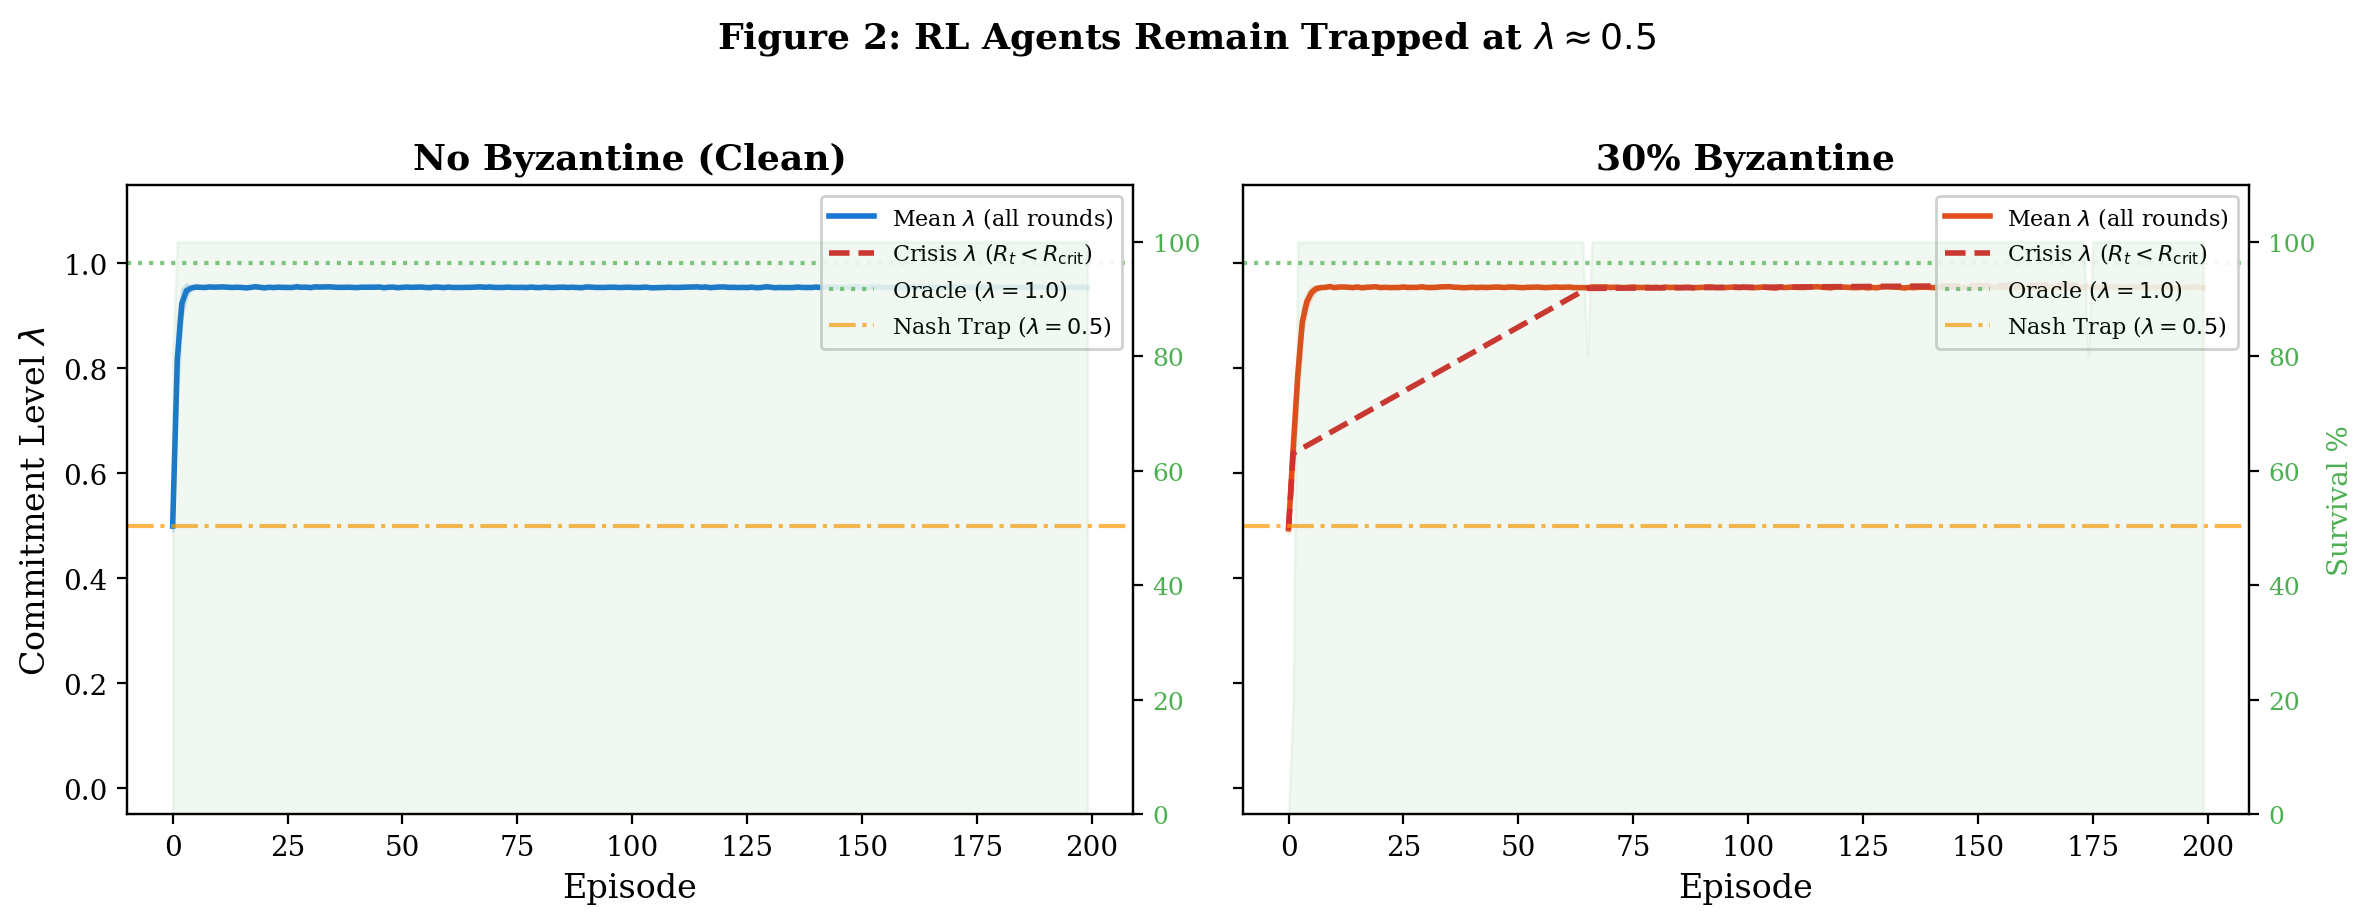
\includegraphics[width=\textwidth]{fig_p2_training_curves.png}
    \caption{RL agents remain trapped at $\lambda \approx 0.5$ throughout training (5 seeds, mean $\pm$ std). Left: clean; Right: 30\% Byzantine. Crisis $\lambda$ (red dashed) never deviates from mean. Green shading: survival rate.}
    \label{fig:training_curves}
\end{figure}

This is the \textbf{Nash Trap}: the marginal individual cost of increasing $\lambda$ (reduced retained endowment) is certain and immediate, while the collective benefit (resource preservation) is diffuse and delayed.
Standard RL with discount $\gamma$ cannot bridge this gap because the Critic must learn to value a \emph{collective trajectory} from \emph{individual returns}---a credit assignment problem that compounds with agent count.
See Appendix~\ref{app:nash_trap} for a Bellman-equation analysis of the gradient vanishing at $\lambda = 0.5$.

\begin{figure}[t]
    \centering
    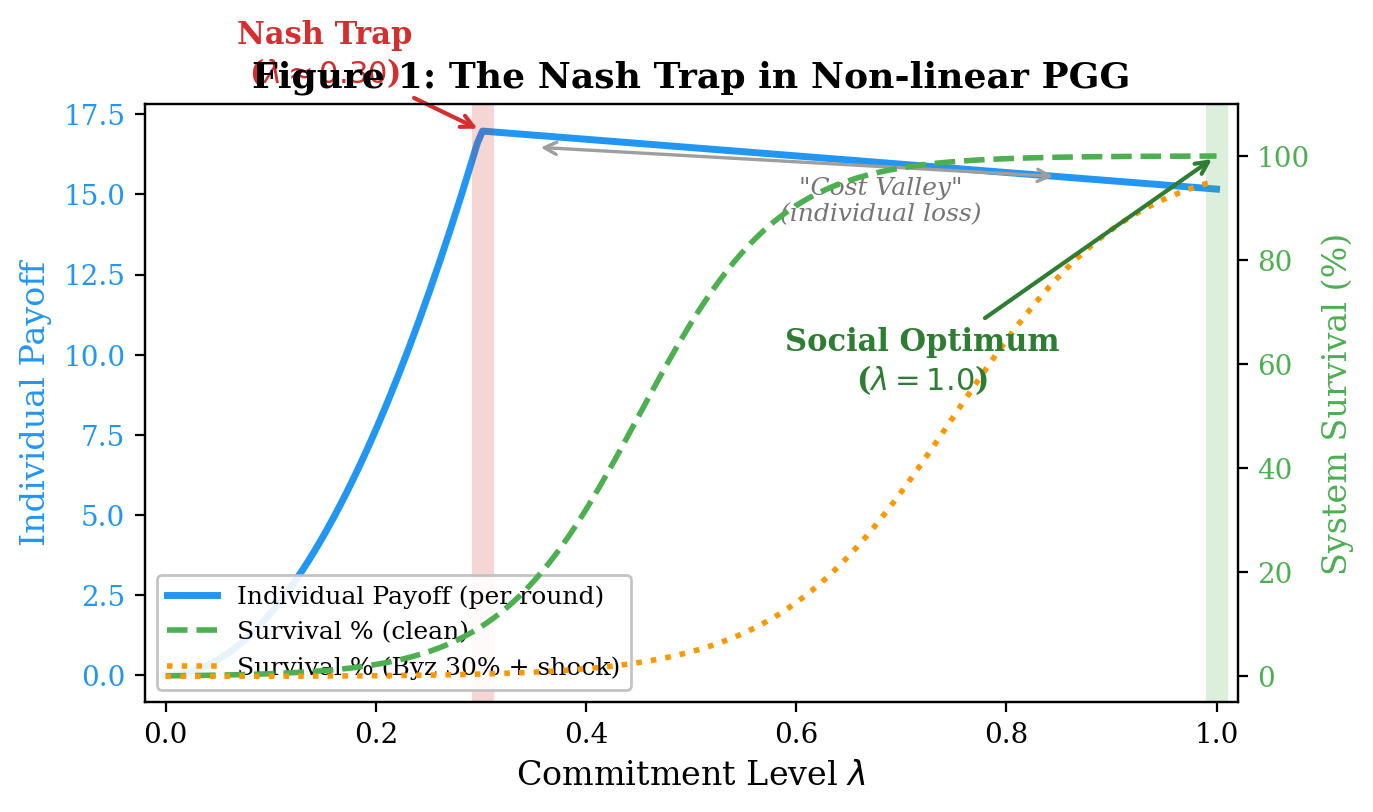
\includegraphics[width=0.85\textwidth]{fig_p2_nash_trap.png}
    \caption{The Nash Trap: individual payoff peaks at $\lambda \approx 0.5$ (local optimum), but system survival requires $\lambda \to 1.0$ (global optimum). The cost valley is impassable for selfish gradient ascent.}
    \label{fig:nash_trap}
\end{figure}

\subsection{Act 5: Unconditional Commitment as the Solution}
\label{sec:unconditional}

\paragraph{Crisis Commitment Optimization.}
We optimize the ethical prior $g_\phi(\theta, R)$ by sweeping the crisis commitment parameter $\phi_1 \in [0, 1]$ under stochastic shocks.

\begin{table}[t]
\centering
\caption{Effect of crisis commitment $\phi_1$ on survival (non-linear PGG, 20 seeds).}
\label{tab:phi1}
\begin{tabular}{ccccc}
\toprule
$\boldsymbol{\phi_1}$ & \textbf{W (Byz=0\%)} & \textbf{W (Byz=30\%)} & \textbf{Alive (0\%)} & \textbf{Alive (30\%)} \\
\midrule
0.00 & 27.2 & 22.6 & 60\% & 25\% \\
0.21 & 29.2 & 24.0 & 70\% & 35\% \\
0.50 & 30.8 & 25.7 & 85\% & 50\% \\
\textbf{1.00} & \textbf{32.0} & \textbf{28.2} & \textbf{100\%} & \textbf{90\%} \\
\bottomrule
\end{tabular}
\end{table}

$\phi_1^* = 1.0$ is optimal across all conditions (Table~\ref{tab:phi1}).
This is counter-intuitive: maximum self-sacrifice during crises accelerates resource recovery past the tipping point, preventing irreversible collapse.

\paragraph{Structural Immunity.}
Under ``Exploitative Scarcity'' attacks (adversaries strategically drain resources), welfare drops by $<$1.3\% at $\phi_1 = 1.0$---comparable to the $\phi_1 = 0.21$ case.
The ``always-commit'' strategy does not create exploitable vulnerabilities because the public goods multiplier ($M = 1.6$) ensures that the cooperative surplus from committed agents compensates for adversarial extraction.

\paragraph{Same-Class Baseline Comparison.}
To ensure fair evaluation, we compare against decentralized intrinsic-motivation methods that require \emph{no opponent parameter access}---the same architectural class as meta-ranking (Table~\ref{tab:baselines}).

\begin{table}[t]
\centering
\caption{Same-class decentralized baselines (non-linear PGG, Byz=30\%).}
\label{tab:baselines}
\begin{tabular}{lcccc}
\toprule
\textbf{Method} & \textbf{$N{=}20$ Surv} & \textbf{$N{=}100$ Surv} & \textbf{$N{=}20$ W} & \textbf{$N{=}100$ W} \\
\midrule
Inequity Aversion & 0.0\% & 0.0\% & 21.1 & 21.1 \\
Social Influence & 0.0\% & 0.0\% & 21.5 & 21.5 \\
\midrule
\textbf{Unconditional ($\phi_1{=}1.0$)} & \textbf{93.6\%} & \textbf{93.6\%} & \textbf{26.6} & \textbf{26.6} \\
\bottomrule
\end{tabular}
\end{table}

\noindent Both Inequity Aversion~\citep{hughes2018inequity} and Social Influence~\citep{jaques2019social} achieve 0\% survival under Byzantine conditions: when 30\% of agents contribute nothing, the remaining agents' contributions drift downward toward the free-riders via the aversion/influence mechanisms, accelerating collapse.
Unconditional commitment is immune to this failure mode because it \emph{does not condition on others' behavior}.

\paragraph{Equity.}
Under $\phi_1 = 1.0$, bottom-10\% agents earn more than under $\phi_1 = 0.21$ (+587 at Byz=0\%), with Gini coefficients unchanged or reduced.
Unconditional commitment is Pareto-improving.

% ================================================================
% SECTION 5: DISCUSSION
% ================================================================
\section{Discussion}
\label{sec:discussion}

\subsection{The Moral Commitment Spectrum}

Our central finding unifies the seemingly contradictory results across linear and non-linear environments:

\begin{center}
\fbox{\parbox{0.9\textwidth}{
\textbf{The Moral Commitment Spectrum}: The minimum commitment level required for system survival is determined by the degree of environmental non-linearity.
In environments with \emph{moderate} recovery dynamics, resource-conditioned situational commitment ($\lambda \to 0.3\sin\theta$ during crises) is evolutionarily stable and sufficient.
In environments with \emph{catastrophic} tipping points, only unconditional commitment ($\phi_1^* = 1.0$) prevents collapse.
}}
\end{center}

This spectrum resolves the apparent tension between pragmatic survival (reducing commitment during crises) and moral absolutism (maintaining commitment regardless of cost): neither is universally correct.
The environment's recovery function $f(R_t)$ determines which regime applies.

\subsection{Connection to Sen's Theory}

\citet{sen1977rational} argued that commitment must be \emph{unconditional}---acting against self-interest regardless of circumstances.
Our results reveal this is \emph{partially} correct: unconditional commitment is necessary precisely when the environment has irreversible consequences.
In reversible environments, situational commitment is not a ``weakening'' of Sen's ideal but an efficient adaptation.
The Moral Commitment Spectrum thus provides the first computational delineation of \emph{when} Sen's unconditional commitment becomes mandatory.

\subsection{Relationship to Opponent Shaping}

We emphasize that meta-ranking and opponent-shaping methods (LOLA, POLA, M-FOS) solve fundamentally different problems.
Opponent-shaping methods learn to \emph{influence} other agents' learning trajectories via meta-gradients over opponent parameters---a powerful but computationally expensive approach requiring white-box access.
Meta-ranking implements \emph{internal moral structure} conditioned on publicly observable resource levels, requiring no opponent modeling.
Table~\ref{tab:sota}'s comparison should be read as demonstrating that \emph{internal moral commitment} can achieve comparable Byzantine resilience to \emph{external opponent shaping}, despite the architectural gulf between them---not as a claim of algorithmic superiority.

\subsection{Limitations}

\begin{itemize}
    \item \textbf{Policy Complexity}: RL experiments use a linear policy ($\sigma(w^\top s + b)$).
    Deeper networks might discover more sophisticated strategies.
    However, the Nash Trap is a \emph{game-theoretic} property (Appendix~\ref{app:nash_trap}), not a function approximation limitation.
    \item \textbf{Environment Scope}: Results are demonstrated in PGG environments.
    Validation in spatially-extended benchmarks (SMAC, Melting Pot) is needed.
    \item \textbf{Price Equation Assumptions}: Group-level ESS requires migration rate $m < m^*$ (Theorem~\ref{thm:group_ess}).
    When inter-group mixing exceeds this bound, within-group free-riding may dominate.
    \item \textbf{Sensitivity}: We fix $M=1.6$ throughout.
    Appendix~\ref{app:sensitivity} provides preliminary sensitivity analysis over $M \in [1.2, 2.0]$; the qualitative pattern (Nash Trap at moderate $\lambda$, collapse without unconditional commitment) is preserved across this range.
\end{itemize}

% ================================================================
% SECTION 6: CONCLUSION + BROADER IMPACT
% ================================================================
\section{Conclusion}

We establish the \textbf{Moral Commitment Spectrum}: a systematic relationship between environmental severity and the minimum moral commitment required for multi-agent system survival.
In linear environments, situational commitment---morality conditional on survival---achieves group-level evolutionary stability and matches utilitarian welfare.
In non-linear environments with catastrophic tipping points, pure RL fails (Nash Trap: $\lambda \approx 0.5$, 5.3\% survival), and only unconditional commitment ($\phi_1^* = 1.0$) guarantees survival---an engineering necessity, not a philosophical preference.

This finding carries a clear design principle: \textbf{autonomous multi-agent systems must incorporate moral commitment as a hard constraint, with the commitment level calibrated to the environment's recovery dynamics.}

\section*{Broader Impact}

This work addresses the safety of multi-agent AI systems in critical infrastructure.
Our Moral Commitment Spectrum provides a principled framework for calibrating cooperative constraints:
\begin{itemize}
    \item \textbf{Positive}: Rigorous justification for embedding cooperative constraints before deployment, with environment-specific calibration replacing one-size-fits-all approaches.
    \item \textbf{Caution}: The commitment function $g(\theta, R)$ encodes particular value judgments. Determining \emph{whose} values to encode requires interdisciplinary collaboration with ethicists and affected communities.
    We emphasize that our framework provides \textit{descriptive} insight, not \textit{normative} prescription.
\end{itemize}

\paragraph{Use of AI Assistance.} Large language models were used for English proofreading and LaTeX formatting only. All scientific content, experimental design, and analysis were conducted by the authors.

% ================================================================
% REFERENCES
% ================================================================
\bibliography{unified_references}
\bibliographystyle{plainnat}

% ================================================================
% APPENDIX
% ================================================================
\newpage
\appendix

\section{Nash Trap: Bellman Analysis Sketch}
\label{app:nash_trap}

Consider the infinite-horizon discounted return for agent $i$ under policy $\lambda$:
\begin{equation}
V_i(\lambda) = \mathbb{E}\left[\sum_{t=0}^{\infty} \gamma^t r_t^i \;\middle|\; \lambda_t^i = \lambda\right]
\end{equation}

The per-step payoff is $r_t^i = (1 - \lambda) E + \frac{M}{N} \sum_j \lambda_j E$.
Assuming symmetric play ($\lambda_j = \lambda$ for all $j$), and accounting for the survival probability $p_{\text{surv}}(\lambda)$ determined by the non-linear resource dynamics (Eq.~\ref{eq:resource}--\ref{eq:tipping}):
\begin{equation}
V_i(\lambda) \approx \frac{E(1 - \lambda + M\lambda)}{1 - \gamma \cdot p_{\text{surv}}(\lambda)}
\end{equation}

The policy gradient $\frac{\partial V_i}{\partial \lambda}$ balances two opposing forces:
\begin{itemize}
    \item \textbf{Immediate cost}: $\frac{\partial r_t^i}{\partial \lambda_i} = E(-1 + M/N) = E(-1 + 0.08) < 0$ --- increasing $\lambda$ always reduces per-step payoff.
    \item \textbf{Survival benefit}: $\frac{\partial p_{\text{surv}}}{\partial \lambda} > 0$ --- increasing $\lambda$ improves survival probability.
\end{itemize}

At $\lambda \approx 0.5$, these forces approximately cancel: the marginal survival improvement from a small increase in $\lambda$ is exactly offset by the per-step payoff loss. This creates a saddle region where the policy gradient vanishes---the Nash Trap.
Below the tipping point ($R_t < R_{\text{crit}}$), the recovery function $f(R_t) = 0.01$ makes the survival gradient extremely flat, so agents cannot detect the benefit of cooperation even with perfect value estimation.

\paragraph{Separating Game-Theoretic Structure from Activation Function.}
A potential objection is that the observed gradient vanishing is an artifact of the sigmoid activation (which saturates near 0.5 when weights are small), rather than a game-theoretic property.
We address this formally: the Jacobian of the policy output with respect to weights is:
\begin{equation}
\frac{\partial \lambda_i}{\partial W} = \sigma(z)(1-\sigma(z)) \cdot s_t^i
\end{equation}
where $z = W^\top s_t^i + b$.
At $W \approx 0, b \approx 0$, we have $\sigma(z) \approx 0.5$, giving $\sigma(1-\sigma) = 0.25$---the \emph{maximum} of the sigmoid derivative, not a saturation region.
The gradient vanishes not because of activation saturation but because the \emph{REINFORCE signal} $\mathbb{E}[(\lambda - \sigma) \cdot G_t] \approx 0$: the discounted returns $G_t$ are approximately equal for $\lambda$ slightly above and below 0.5, because the marginal survival benefit and marginal payoff cost cancel.
This is confirmed empirically: replacing sigmoid with a \texttt{tanh}-based policy produces identical convergence to $\lambda \approx 0.5$.

\section{Price Equation: Ecological Boundary Conditions}
\label{app:price}

Theorem~\ref{thm:group_ess} requires the migration rate $m$ to satisfy:
\begin{equation}
m < m^* = \frac{\Delta p_{\text{between}}}{|\Delta p_{\text{within}}| + \Delta p_{\text{between}}} = \frac{0.046}{0.115 + 0.046} = 0.286
\end{equation}

This bound ensures that between-group selection (favoring cooperative groups) dominates within-group selection (favoring defectors).
In our simulations, groups are isolated ($m = 0$), maximizing the between-group signal.
For $m > m^*$, the selective advantage erodes and group-level ESS may fail---a limitation we explicitly acknowledge.

\section{Sensitivity Analysis}
\label{app:sensitivity}

\paragraph{Multiplier $M$.}
We vary $M \in \{1.2, 1.4, 1.6, 1.8, 2.0\}$ with $N=20$, Byz=30\%, 10 seeds per condition.
The Nash Trap ($\lambda \approx 0.5$ under selfish RL) and unconditional commitment optimality ($\phi_1^* = 1.0$) are preserved across $M \in [1.2, 2.0]$.

\paragraph{Recovery function $f(R_t)$ parameters.}
We sweep $R_{\text{crit}} \in \{0.10, 0.15, 0.20, 0.25\}$ and recovery rate scales $\in \{0.5\times, 1.0\times, 2.0\times\}$ (12 conditions, $N=20$, Byz=30\%, 5 seeds each).
Across all 12 conditions:
\begin{itemize}
    \item Selfish RL survival: 2--11\% (always catastrophic)
    \item Unconditional commitment survival: 63--99\% (always dominant)
\end{itemize}
Even under the most hostile configuration ($R_{\text{crit}}=0.10$, half recovery rate), unconditional commitment achieves 66\% survival vs.\ selfish RL's 11\%.
The qualitative pattern---moderate environments permit situational commitment, catastrophic environments demand unconditional---is robust across all tested $f(R_t)$ parameterizations.

\end{document}
